\subsection{Setzeinheit} \label{sec:Setzeinheit}
\textit{(ygu)} Die Setzeinheit bezeichnet alle Teile, welche durch die Translation bewegt werden. Auch zur Setzeinheit gehören die Spindel sowie der Spindelantrieb, welche die Translation umsetzen.
\newline
Die wesentlichen Komponenten der Setzeinheit sind in Abbildung \ref{fig:setzeinheit} dargestellt. Dabei wird in diesem Unterkapitel ausschliesslich auf die Komponenten der Setzeinheit eingegangen. Alle Komponenten die zur Verstellung des Topfradius dienen, sind in der Abb.  \ref{fig:setzeinheit} unter Punkt 8 (Verstellmechanik) gesammelt und werden im Kapitel \ref{verstellmechanik} näher erläutert.
\subsubsection{Aufbau}
Die Spindel ist durch eine bewegte Montageplatte (Punkt. 16 in Abb. \ref{fig:setzeinheit}) und drei Führungen (6) mit der Verstellmechanik (8) verbunden. Diese Führungen werden durch drei Gleitlager (7)  an einer Montageplatte (14) gelagert. die zwei oberen Montageplatten (12, 13) dienen zur Montage des Spindelantriebes sowie zur Lagerung der Spindel (4). Um eine weitere Montageplatte zu sparen, ist der Spindelantrieb mittels einer Distanzhülse (2) mit der obersten Montageplatte (12) verbunden. Die unterste Montageplatte (15) dient zur Lagerung der Verstellmechanik sowie zum einfachen Schutz der Mechanik vor Topferde. Dadurch ist gewährleistet, dass nur ein minimaler Teil (der Stechdorn, 9 - 11) der bewegten Komponenten in Kontakt mit der Topferde kommt.
	\begin{figure}[H]
	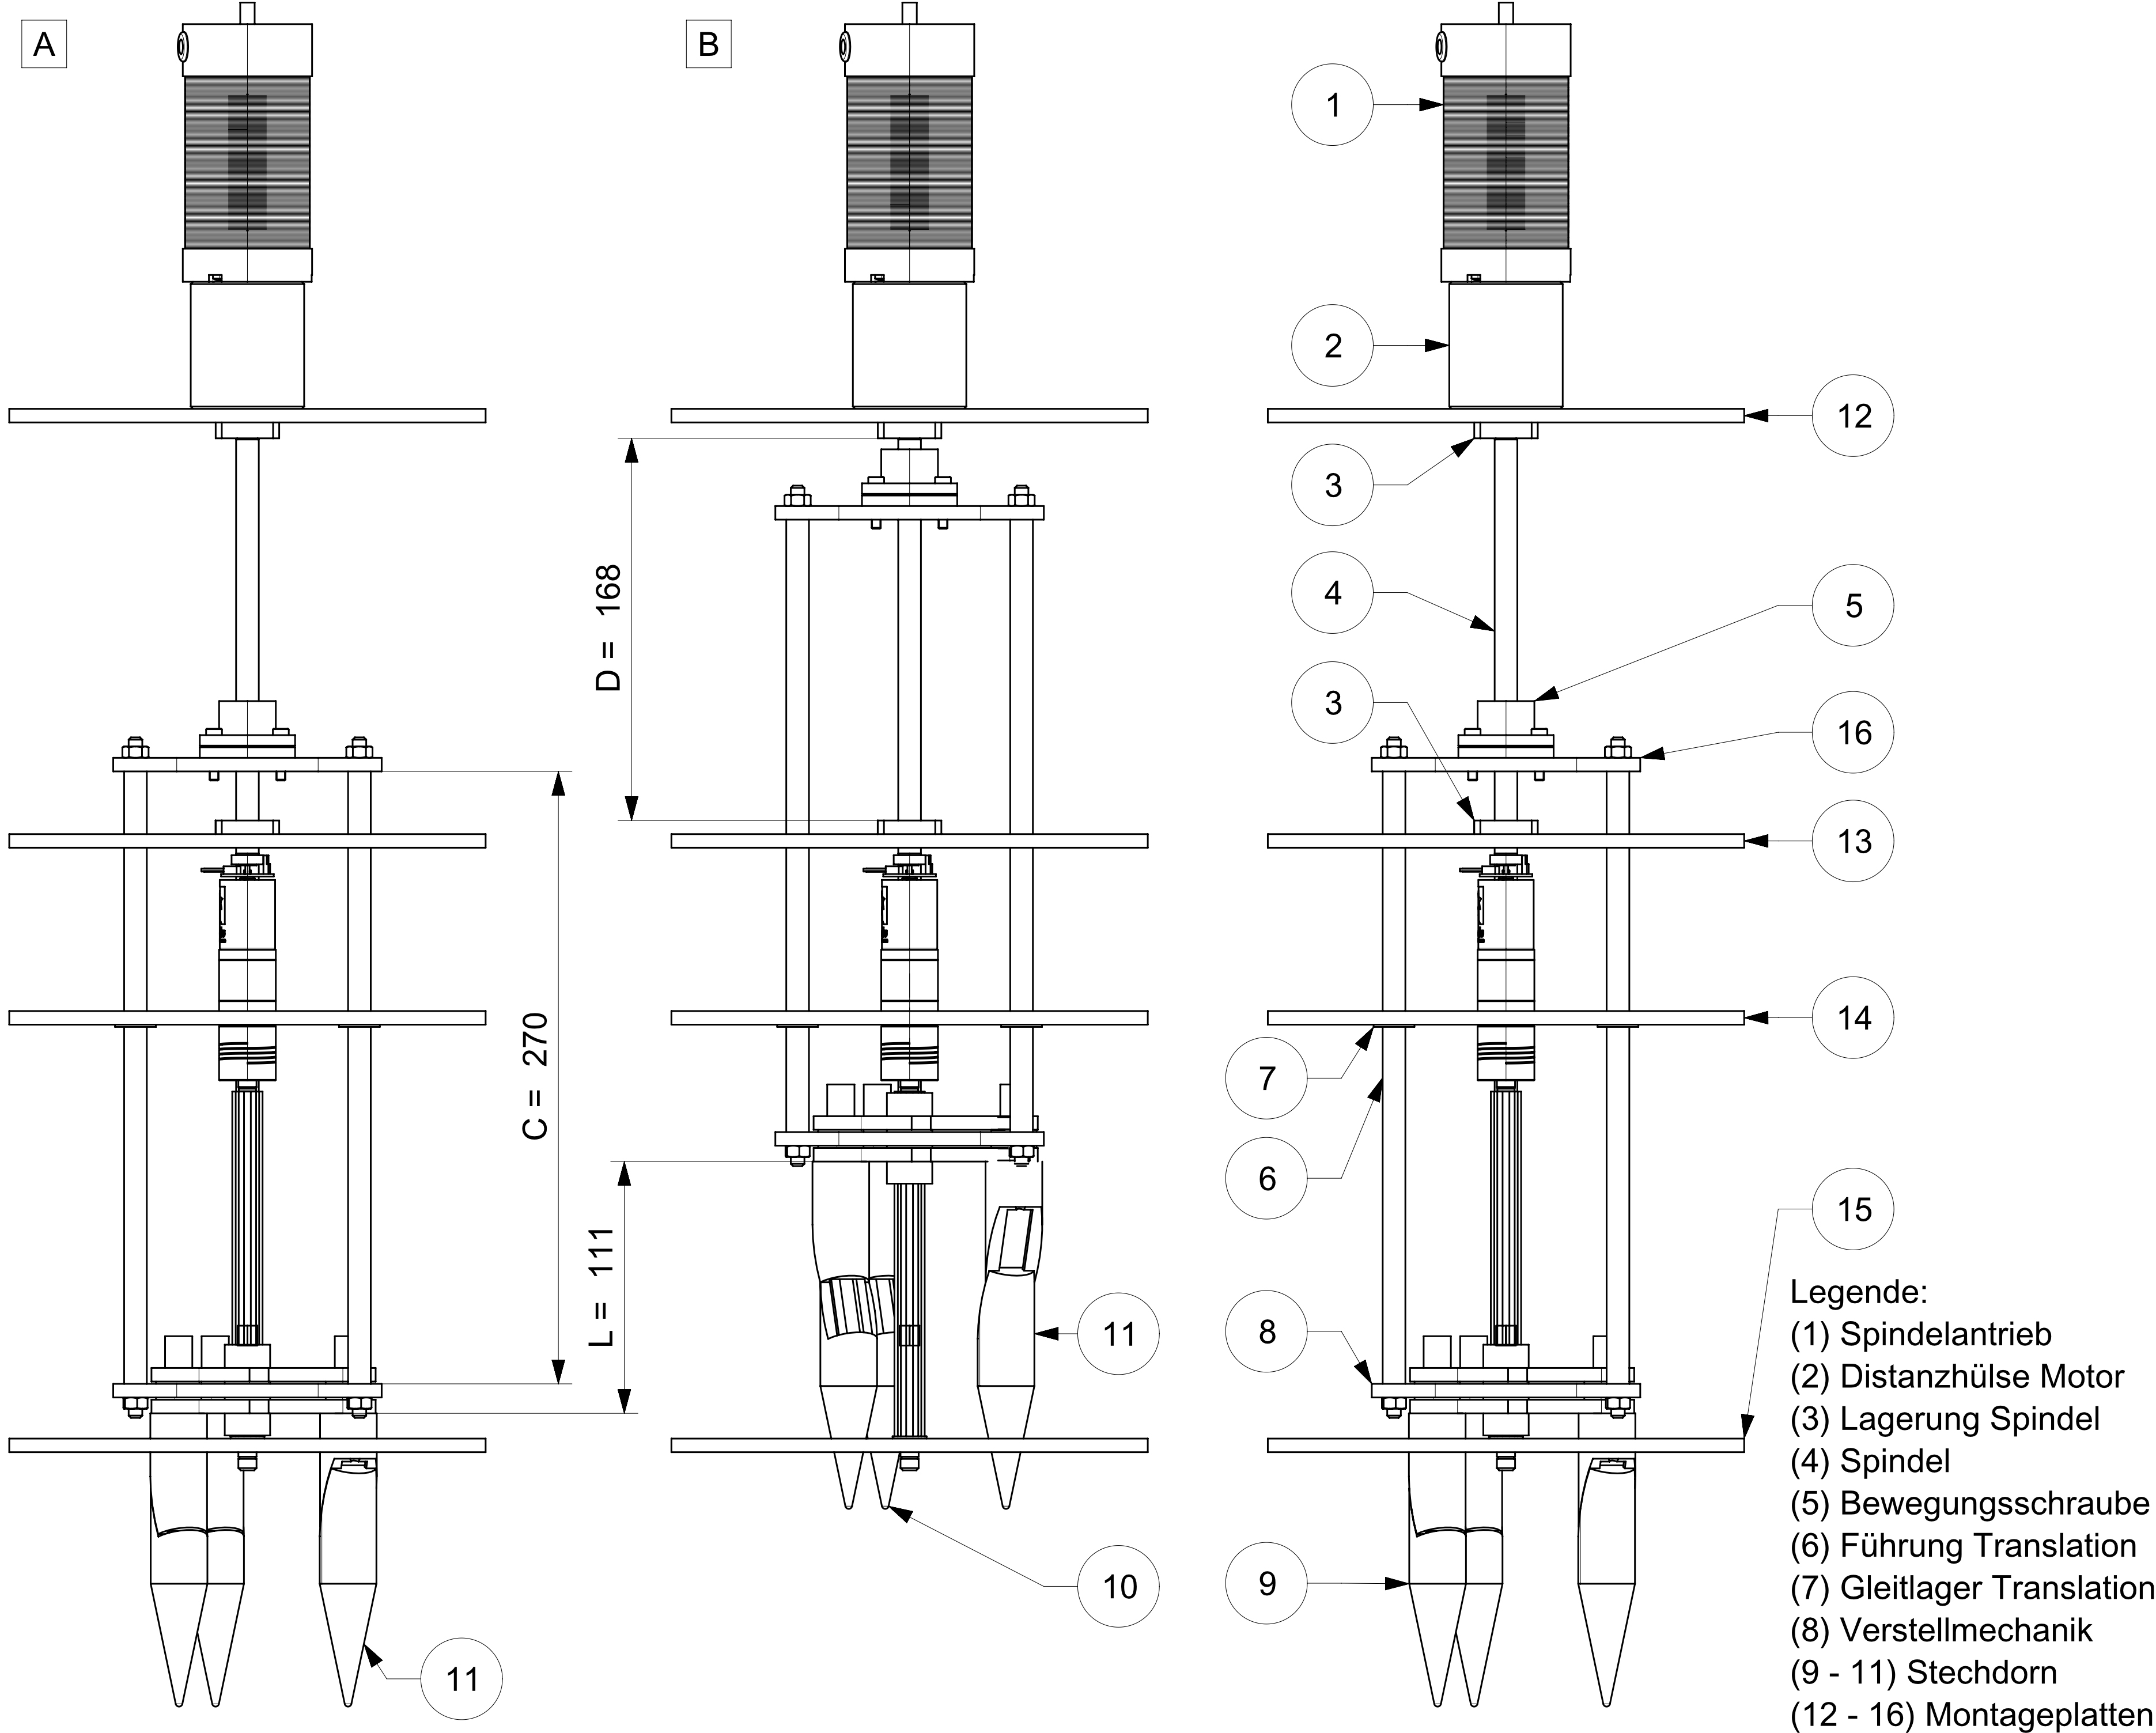
\includegraphics[scale=0.53]{Illustrationen/6-Umsetzung/setzeinheit_aio.jpg}
	\caption{Detaillierte Übersicht der Setzeinheit}
	\label{fig:setzeinheit}
\end{figure}

 
\subsubsection{Translation der Setzeinheit}
Um drei NemaCaps in einen Topf zu pflanzen, erfolgt folgender Prozess:
\begin{itemize}
	\item \textbf{A - Setzloch ausheben:} Die Spindel bewegt die Setzeinheit nach unten und treibt den Stechdorn in die Erde. Dadurch verschliesst sich der Stechdorn (Punkt 11 in Abb. \ref{fig:setzeinheit}). 

	\item \textbf{B - NemaCap setzen:} Nachdem die Erde verdrängt und das Setzloch ausgehoben ist, bewegt sich die Setzeinheit wieder nach oben. Nun öffnet sich der Stechdorn (10) indem sich der untere Teil durch die Schwerkraft seitlich nach unten bewegt. So können die NemaCaps in das ausgehobene Setzloch fallen.
\end{itemize}
\newpage
Konstruktiv sind drei Masse hervorzuheben:
\begin{itemize}
	\item \textbf{L - Maximaler Hubweg:} Der maximale Hub L beträgt 111mm. Gemäss Berechnungen (vgl. Anhang 'Auslegung Spindel') muss dieser mindestens 86mm betragen. Somit beträgt die Reserve 25mm. 
	
	\item \textbf{C - Länge der Führungen:} Die Länge der Führungen ist durch den Hubweg L gegeben, der Höhe des Motors für die Verstellmechanik  und dessen Kupplung. Dies bedingt eine Länge von 270mm.
	
	\item \textbf{D - Länge der Spindel:} Die Spindellänge ergibt sich durch den maximalen Hub L und der Höhe der Bewegungsschraube (Punkt 5 in Abbildung \ref{fig:setzeinheit}) plus Montageplatte (15). Dadurch beträgt die Länge der Spindel 168mm.
\end{itemize}

\subsubsection{Spindel} \label{sec:Umsetzung_Spindel}
Die Wahl der Spindel und des Spindelantriebes haben einen entscheidenden Einfluss auf die Erfüllung des Setzprozesses innerhalb der vorgegeben Zeit. Parameter wie Steigung, Spindeldurchmesser und Material der Spindel wirken sich direkt auf die Massenträgheit und somit auf das erforderliche Beschleunigungsmoment aus.
\newline

Dieses Subkapitel befasst sich mit der Auslegung und Berechnung der Spindel. Dabei sind Berechnungen in zusammengefasster Form dargestellt. Der vollständige Rechenweg und die detaillierte Vorgehensweise sind im Anhang (Dokument \textit{Auslegung Spindel}) zu entnehmen.

Folgende Daten sind durch den Setzprozess und die Geometrie gegeben:
	\begin{figure}[H]
	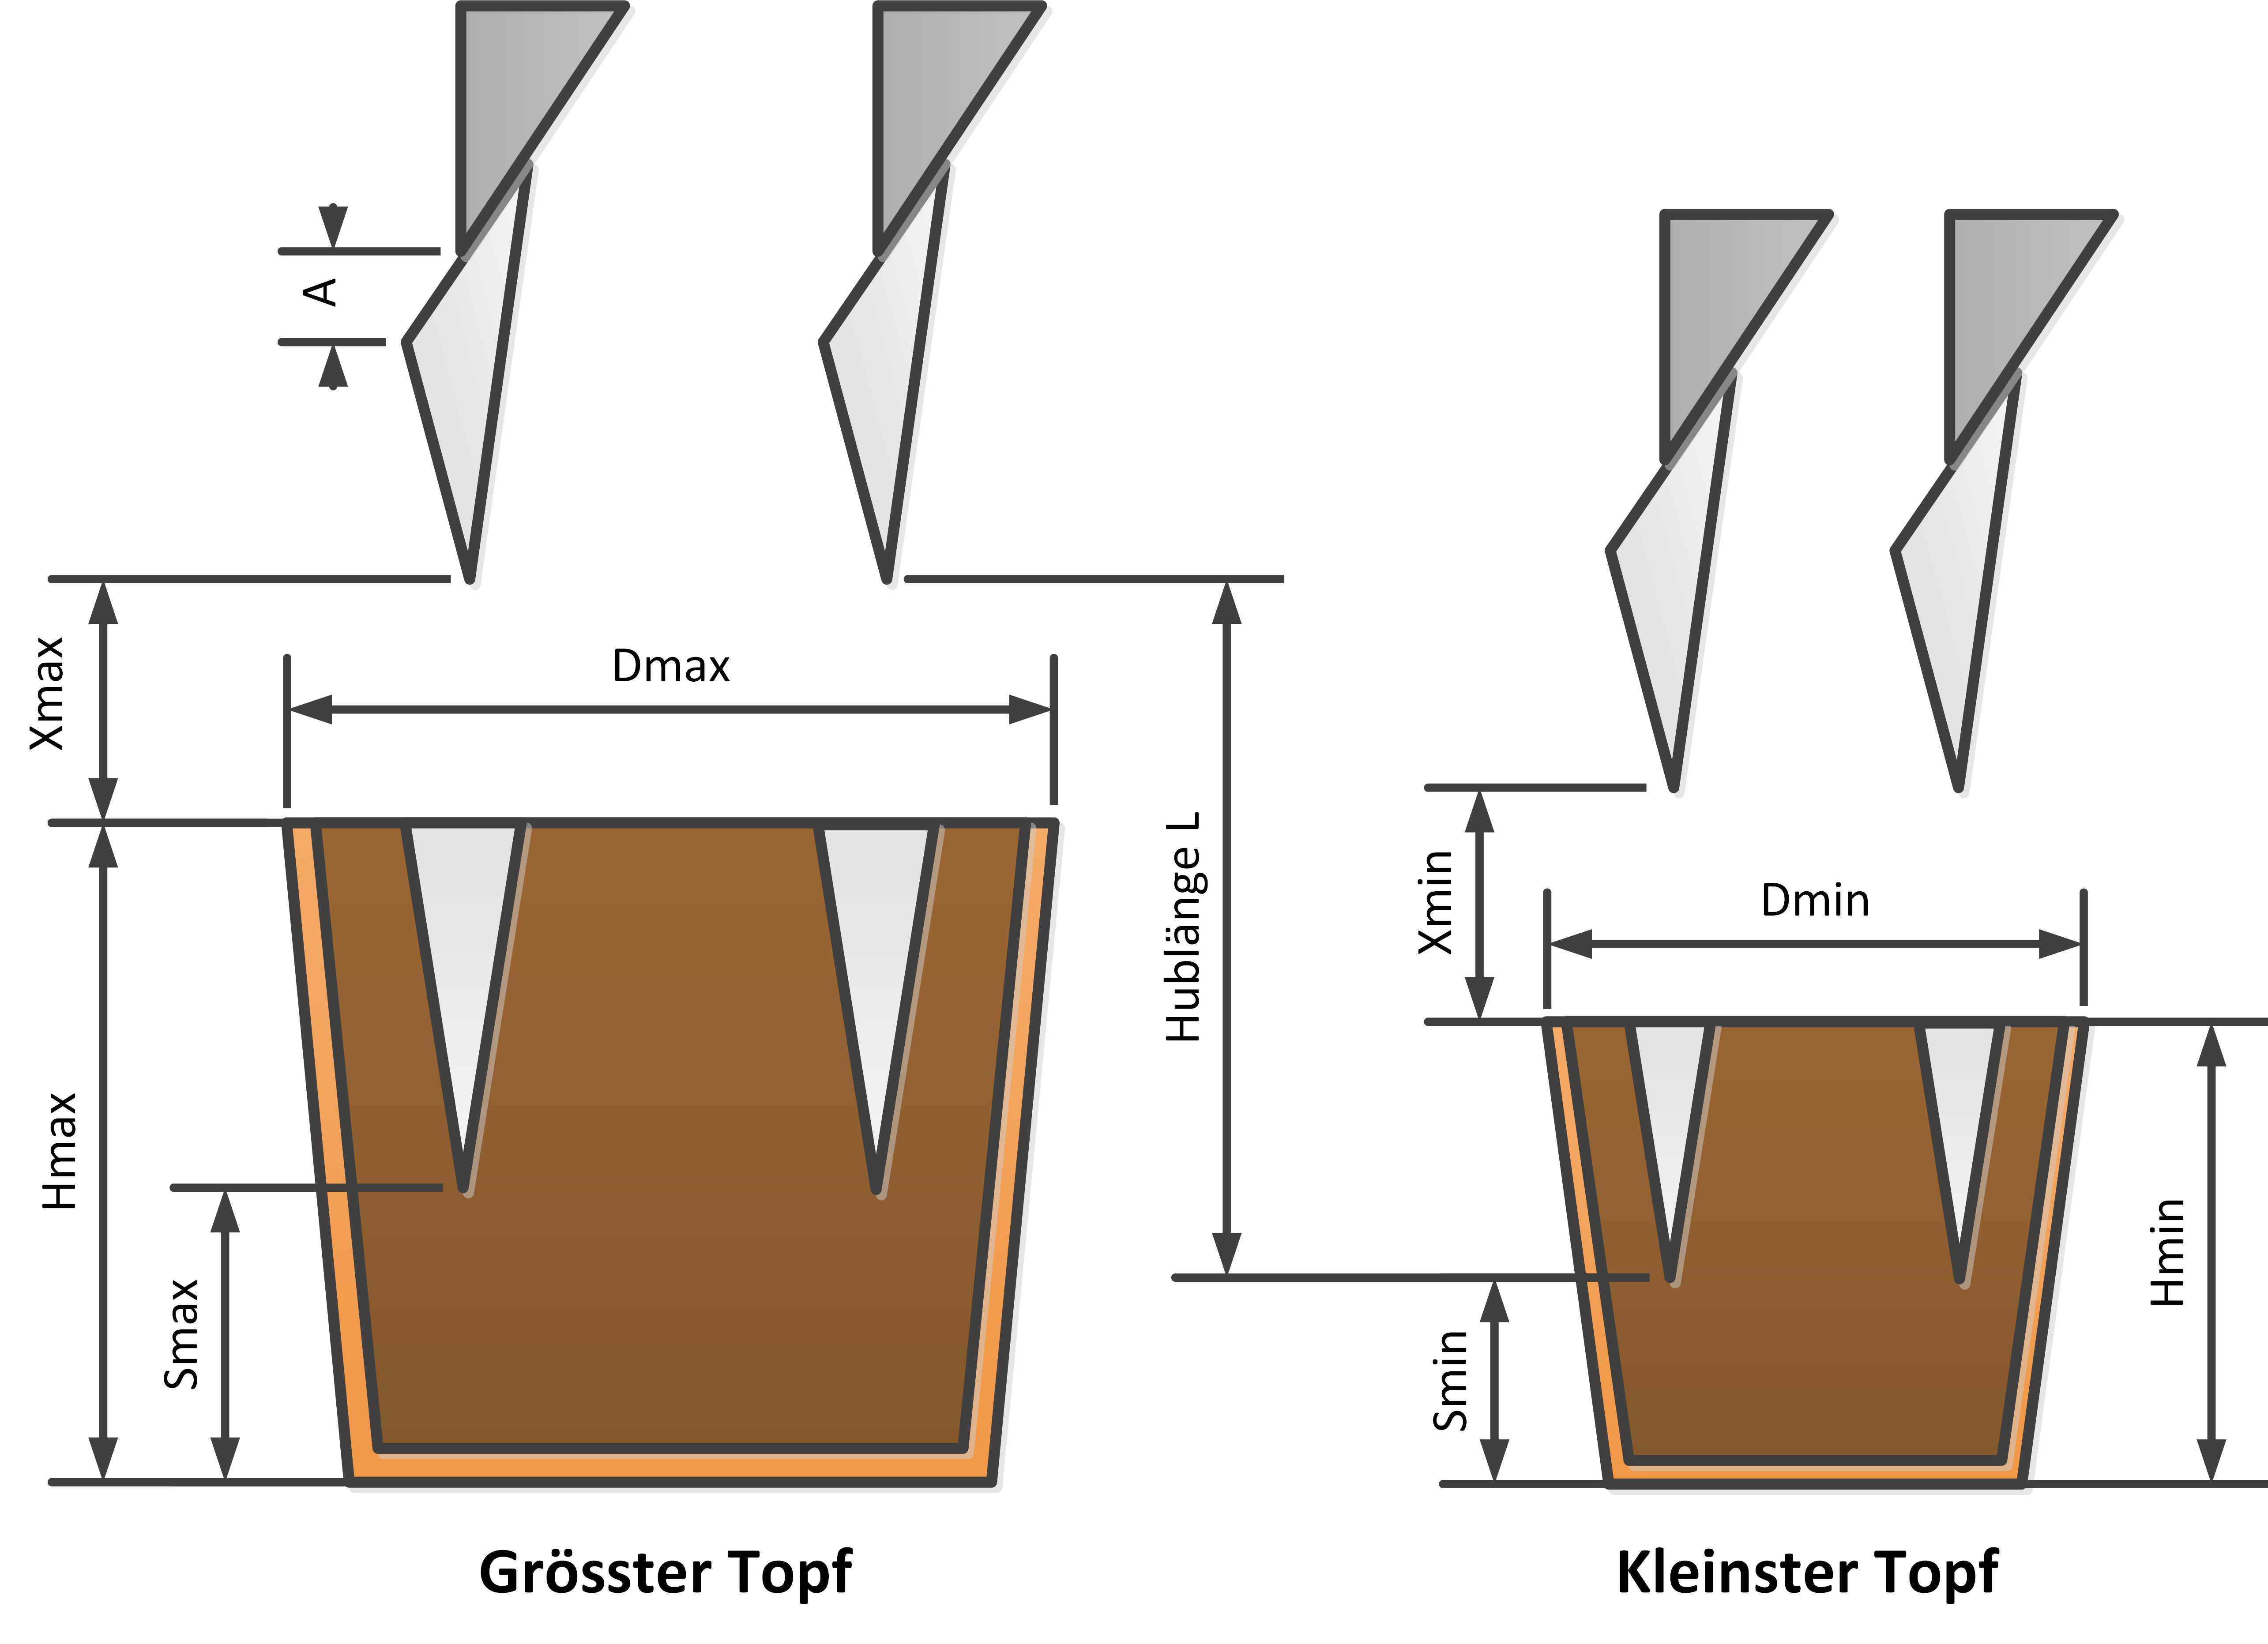
\includegraphics[width=1\textwidth]{Illustrationen/6-Umsetzung/topfgeometrie.png}
	\caption{Geometrie der Töpfe und des Setzprozess}
	\label{fig:topfgeometrie}
	\end{figure}
\begin{table}[H]
	\small
\begin{tabular}{|l|c|c|l|}
	\hline 
	& Grösster Topf (max) & Kleinster Topf (min) & Kommentar \\ 
	\hline 
	Durchmesser D [mm] & 140 & 90 & Aus Datenblatt \\ 
	\hline 
	Höhe h [mm] & 106 & 67 & Aus Datenblatt \\ 
	\hline 
	max. Einsetztiefe S [mm] & 63.6 & 40.2 & 0.6 x Höhe \\ 
	\hline 
	Sicherheitsabstand X [mm] & 15 & 15 & Annahme \\ 
	\hline 
	Ausfahrlänge A Dorn [mm] & 15 & 15 & Annahme \\ 
	\hline 
\end{tabular} 
	\caption{Randbedingungen für Spindelauslegung}
	\label{tab:Randbedingungen}
\end{table}

Anhand dieser Randbedingungen und den getroffenen Annahmen ergeben sich eine Beschleunigungs- und Bremszeit t\textsubscript{b}=0.1125s. Bei einem maximalen Hubweg U\textsubscript{max} = 72.4mm beträgt die grösste durschnittliche Geschwindigkeit v\textsubscript{avmax}:

\begin{equation}
v_{avmax}=\frac{U_{max}}{t_{b}}=\frac{72.4mm}{0.1125s}=643.5mm/s
\end{equation}
\newpage
Die Geschwindigkeit des Dornes kann  gemäss Abbildung \ref{fig:vprofil_dorn} streng idealisiert dargestellt werden:
	\begin{figure}[H]
	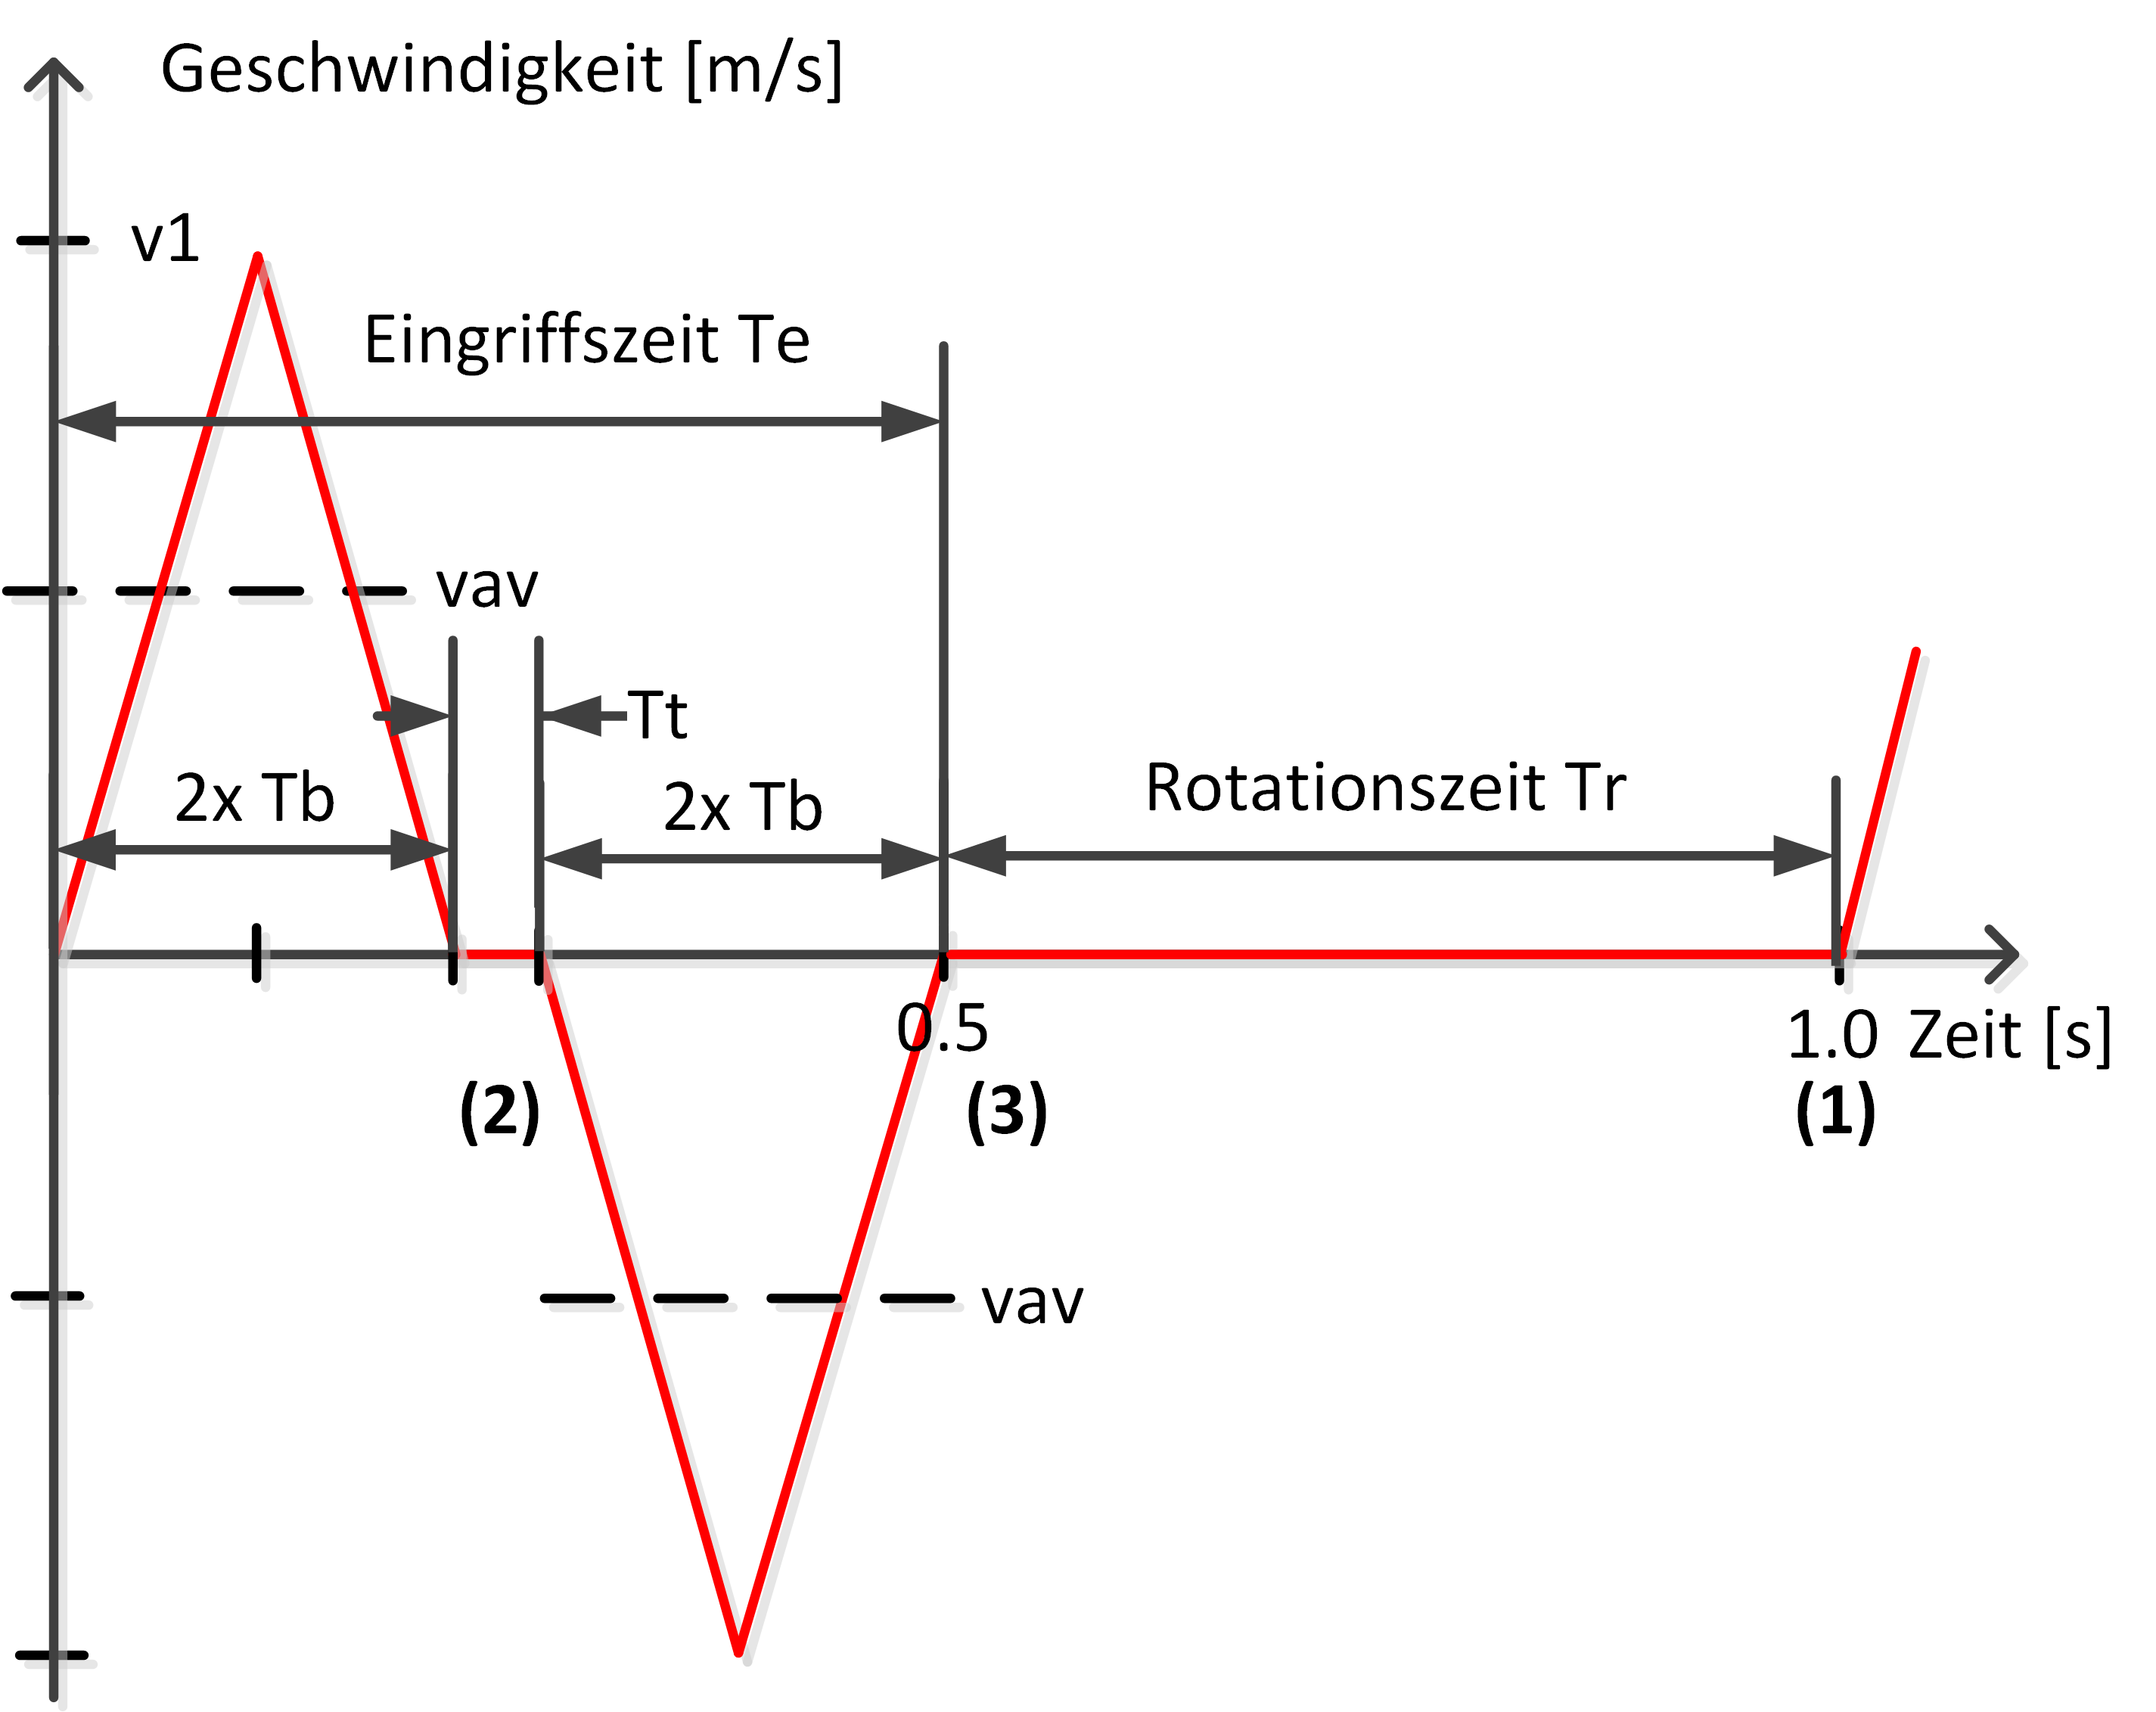
\includegraphics[width=1\textwidth]{Illustrationen/6-Umsetzung/vprofil_dorn.png}
	\caption{Geschwindigkeitsprofil des Dorns}
	\label{fig:vprofil_dorn}
\end{figure}
Basierend auf den Anforderungen aus \ref{subsec:Translation} und der berechneten Geschwindigkeit sind vier Steilgewindespindeln von Igus ausgewählt worden \cite{igusDryspin}. In Rücksprache mit Mark Chalençon, Produktmanager bei Igus Schweiz GmbH, wurde die Auswahl der Produkte zusätzlich verifiziert. 
\begin{table}[H]
\begin{tabular}{|c|c|}
	\hline 
	Ds14x30 (Edelstahl) & Ds10x25 (Edelstahl) \\ 
	\hline 
	Ds14x30 (Aluminium) & Ds10x25 (Aluminium) \\ 
	\hline 
\end{tabular} 
\caption{Ausgewählte Steilgewindespindeln von Igus}
\label{tab:spindeln}
\end{table}
Mit diesen Angaben kann die Spindel durch ein reduziertes Model dargestellt werden, analog zu Abbildung 13-5 (\citeNP[S.~448]{roloffmatek}):
 	\begin{figure}[H]
 	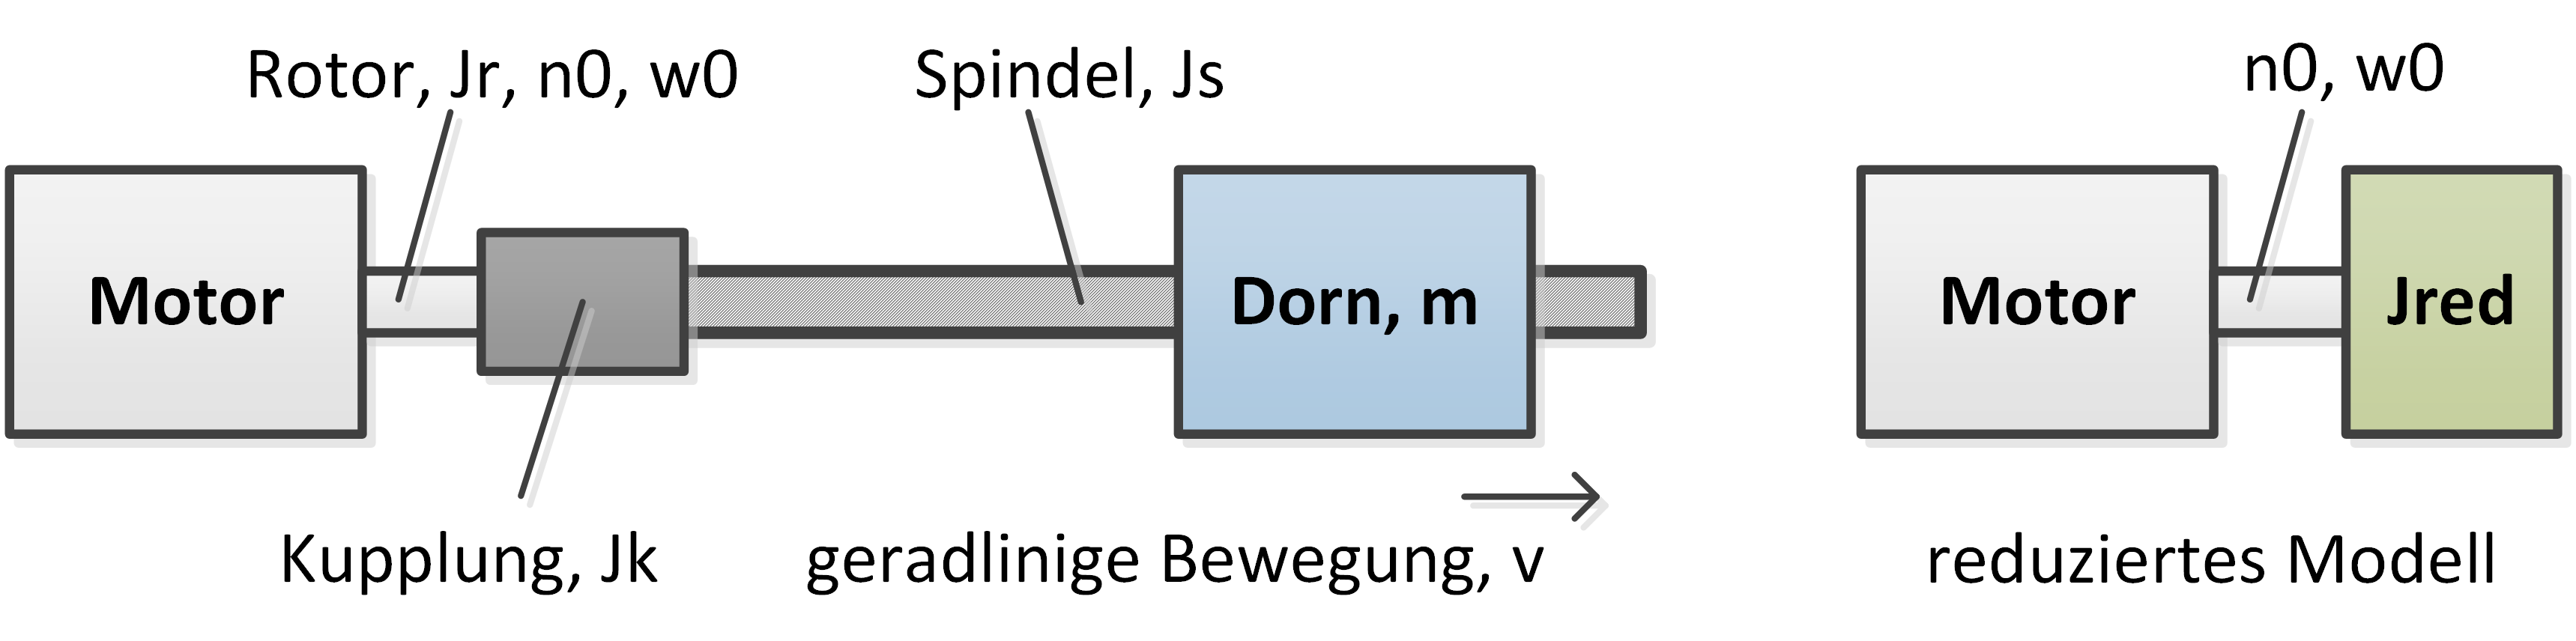
\includegraphics[width=1\textwidth]{Illustrationen/6-Umsetzung/red_modell.png}
 	\caption{Schema des Spindelantriebs sowie des reduzierten Modells}
 	\label{fig:red_modell}
	\end{figure}
Wobei für das reduzierte Modell sich die reduzierte Massenträgheit J\textsubscript{red} und das benötigte Beschleunigungsmoment M\textsubscript{a} ergibt (Gleichung 13.3 und 13.4, S.449):
\begin{equation}
J_{red}=J_{rotor}+J_{kupplung}+J_{spindel}+m*(\frac{v_{1}}{w_{v1}})^{2}
\end{equation}
\begin{equation}
M_{a}=J_{red}*\frac{w_{2}-w_{1}}{t_{b}}=J_{red}*\frac{w_{v1}}{t_{b}}
\end{equation}
Für die ausgewählten Spindeltypen ergibt dies folgende Werte:

\begin{table}[H]
\begin{tabular}{|c|c|c|}
	\hline 
	& reduzierte Massenträgheit J\textsubscript{red}& Beschleunigungsdrehmoment M\textsubscript{a}\\ 
	\hline 
	Ds14x30 Edelstahl & 5.36E-05 & 0.128 \\ 
	\hline 
	Ds14x30 Aluminium & 4.93E-05 & 0.118 \\ 
	\hline 
	Ds10x25 Edelstahl & 4.16E-05 & 0.120 \\ 
	\hline 
	Ds10x25 Aluminium & 4.05E-05 & 0.116 \\ 
	\hline 
	Einheit & kgm$^2$ & Nm \\ 
	\hline 
\end{tabular} 
\caption{Reduzierte Massenträgheit J\textsubscript{red} und benötigtes Beschleunigungsdrehmoment M\textsubscript{a} der ausgewählten Spindeln}
\label{tab:spindel_final}
\end{table}
Die berechneten Werte für das Beschleunigungsmoment M\textsubscript{a} aus Tabelle \ref{tab:spindel_final} zeigen, dass sich alle ausgewählten Spindeln für den evaluierten Spindelantrieb eignen.
\newline
Als definitive Wahl wird die Spindel \textbf{Ds10x25 aus Edelstahl} ausgewählt. Folgende Argumente sind ausschlaggebend:
	\begin{itemize}
	\item Die Variante Ds10x25 aus Edelstahl bietet das Optimum aus kleinem Durchmesser und hoher Festigkeit. Das leicht höhere Beschleunigungsmoment der Ds10x25 aus Edelstahl zur Ds14x30 wird für eine höhere Festigkeit in Kauf genommen.
	
	\item \ Die geringere Steigung gibt dem Motor mehr Weg (Umdrehungen) zur Beschleunigung.
\end{itemize}
Die Ausgewählte Spindel verfügt somit über eine Reserve S von 3.5 gegenüber dem verfügbaren Beschleunigungsdrehmoment des Antriebs (vgl. Anhang: \textit{Auslegung Spindel}).

\subsubsection{Kupplung}
Als mechanischen Verbindung zwischen Spindelantrieb und Spindel wird eine drehstarre Kupplung verwendet. Dadurch kann eine winkelgetreue Drehmomentenübertragung gewährleistet werden, was für diese Anwendung essentiell ist \cite{dubbel}. Hierfür wird die Kupplung HELICAL WA 20-8-6 aus Aluminium von Ringspann AG verwendet \cite{helical}. Die Wahl eines kleinen Aussendurchmessers (20mm) und ein leichter Werkstoff sind für ein möglichst geringes zusätzliches Trägheitsmoment entscheidend und wurden hier berücksichtigt.

\subsubsection{Lagerung}
\textbf{Rotation der Spindel}
\newline
Die Spindel wird durch ein Fest- sowie ein Loslager eindeutig gelagert. Das Festlager ist in der obersten Montageplatte (Punkt. 12 in Abb. \ref{fig:setzeinheit}) vorgesehen, das Loslager hingegen in der zweiten Montageplatte (13). Diese Anordnung ist bewusst so gewählt, damit das Festlager Axialkräfte aufnimmt und der Spindelantrieb axial unbelastet bleibt. Für die Lagerung werden fertige Lagerböcke von Mädler Norm-Antrieb AG verwendet, welche speziell für Spindeln ausgelegt sind \cite{maedler}. Sie erfordern keinen zusätzlichen Entwicklungsaufwand und können einfach eingebaut werden. An der Spindel wird konstruktiv einen Freistich Form E umgesetzt (vgl. Anhang: \textit{Spindel DST LS 10x25})\cite{vsm}.
\newline

\textbf{Translation der Setzeinheit}
\newline
Die Lagerung der translatorischen Bewegung wird durch drei Gleitlager (Punkt. 7 in Abb. \ref{fig:setzeinheit}) realisiert. Dabei werden diese in die Montageplatte (14) eingepresst. Dafür werden drei Kunststoff Gleitlager iglidur JSM-1012 von igus verwendet. Begründet wird die Wahl dadurch, dass Kunstoffgleitlager schmiermittel- und wartungsfrei sind, geringe Reibwerte und eine hohe Lebensdauer aufweisen. Weiter sind dies Standard-Maschinenelemente und dadurch günstig erhätlich. Weitere Informationen zum Gleitlager sind aus dem Datenblatt zu entnehmen \cite{igusJSM}.


\subsubsection{Montage}
Wie schon mehrfach erläutert werden verschiedenste Komponenten an Montageplatten montiert. Wie aus Abbildung \ref{fig:setzeinheit} ersichtlich, werden die Montageplatten vertikal angeordnet. Diese Anordnung bildet das Gerüst für eine funktionierende Setzeinheit. Mechanisch fixiert werden die Montageplatten durch Aluminium Profile der Firma Kanya AG (weitere Informationen: siehe Kapitel \ref{maschinengestell}), wobei durch die Nut der Profile eine Blechdicke von 6mm vorgegeben ist. Diese Konstruktion bringt folgende Vorteile:
	\begin{itemize}
	\item Komponenten können auf unterschiedlichen Ebenen angeordnet werden. Weiter ist das Hinzufügen von weiteren Komponenten auf einfachste Art realisierbar. Wird eine weitere Komponente benötigt, wird die entsprechende Kontur (z.B. ein Langloch oder Bohrung) vorgesehen und die Komponente kann montiert werden.

	\item Die Fixierung der Montageplatten durch Aluminium-Profile macht die Montage flexibler. Dadurch bleibt die Höhe der einzelnen Platten verstellbar. Auch seitlich können die Platten in eine Richtung verstellt werden.
\end{itemize}
 	\begin{figure}[H]
	\includegraphics[width=1\textwidth]{Illustrationen/6-Umsetzung/Montageplatten.png}
	\caption{Übersicht der Montageplatten}
	\label{fig:montageplatten}
\end{figure}
Die Montageplatten 1 bis 3 aus Abbildung \ref{fig:montageplatten} verfügen über drei Langlöcher (Detail A), welche um jeweils 120° verschoben angeordnet sind. Diese sind für die flexible Führung der Schläuche vorgesehen.

\subsubsection{Prozessablauf}
\textit{(pro)} Die translatorische Bewegung der Setzeinheit stellt hohe Anforderungen an die Dynamik des Antriebmotors und dessen Regelung. Dafür wird ein BLDC Motor von Trinamic mit der passenden Steuerung verwendet. Die Spezifikationen, sowie die Begründung für die Wahl dieser Antriebstechnik sind in Kapitel \ref{kap:Evaluation_der_Komponenten} erläutert. Um die Hubposition der Setzeinheit zu bestimmen wird diese in der Initialisierungsphase an den oberen Anschlag bewegt. Durch das Erreichen des Anschlags steigt die Last am Motor und dessen Stromstärke. Durch den Anstieg des Laststroms wird der Endanschlag vom uC erkannt und die Position der Setzeinheit wird auf den Wert 0 gesetzt. Durch die Hall Sensoren des BLDC Motors können dann die relativen Positionen zum Referenzwert angefahren werden.

Das System initialisiert sich nach einem Neustart einmalig und ist dann für den Betrieb bereit. Der ganze Prozess der Setzeinheit ist in Abb. \ref{fig:Prozessablauf_Setzeinheit} illustriert. Die bewegten Massen der Setzeinheit, unter anderem die Stechdorne, wurden als $"$Masse Translation$"$ zusammengefasst. Der Prozess wurde dabei in fünf Etappen unterteilt welche mit den Ziffern 1... 5 nummeriert sind.

\begin{figure}[H]
	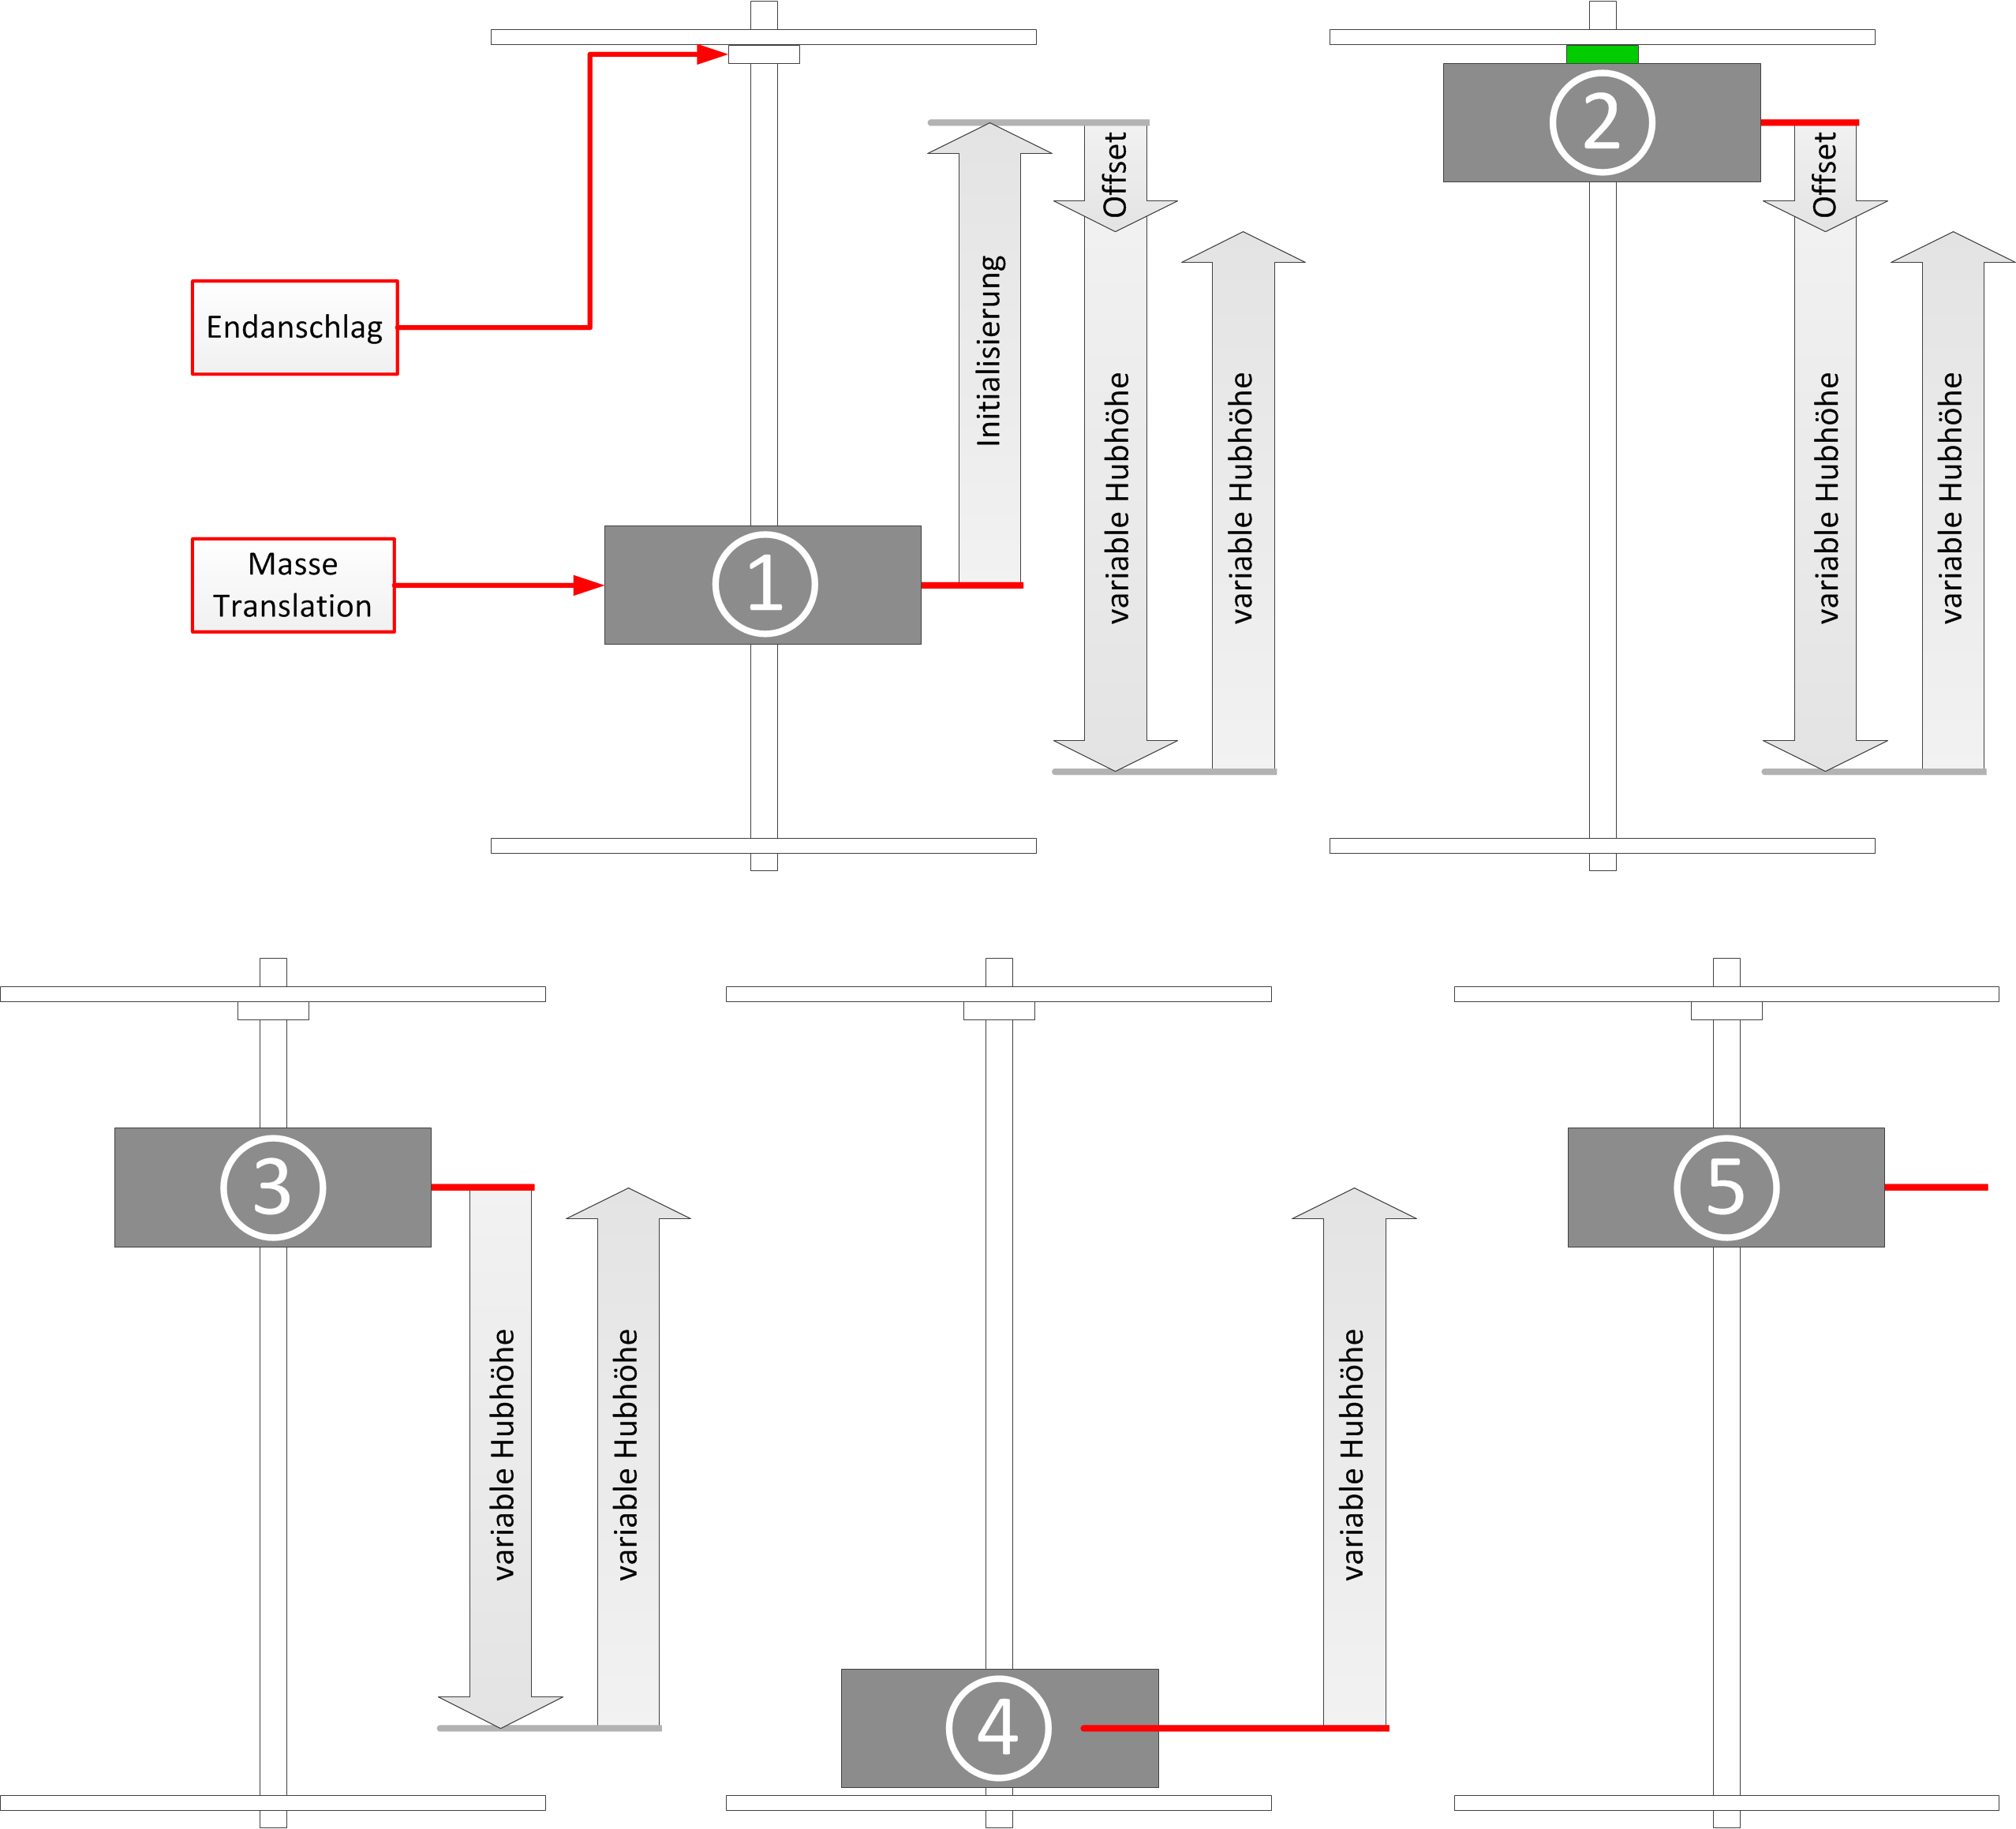
\includegraphics[width=0.9\textwidth]{Illustrationen/6-Umsetzung/Prozessablauf_Setzeinheit.png}
	\caption{Prozessablauf der Setzeinheit}
	\label{fig:Prozessablauf_Setzeinheit}
\end{figure}

Im folgenden Abschnitt werden die fünf Etappen erläutert:

\begin{enumerate}
	\item Die Position des Stechdorns ist nicht bekannt. Die Setzeinheit befindet sich nach einem Neustart des Systems in diesem Zustand. Zu diesem Zeitpunkt wird die Initialisierungsphase gestartet. Die Setzeinheit wird in Richtung des oberen Anschlags bewegt.
	\item Bei Erreichen des oberen Endanschlags wird der Motor angehalten. Um einen gewissen Sicherheitsabstand zwischen der obersten Hubposition der Setzeinheit und dem mechanischen Endanschlag zu gewährleisten, wird die Setzeinheit eine definierte Hubhöhe (Offset) vom Endanschlag wegbewegt. Der Offset kann je nach Topfgrösse ebenfalls angepasst werden, damit sich die Setzeinheit in der Ausgangsposition (Etappe 3) näher an der Topferde befindet und dadurch einen kürzeren Hub fahren muss.
	\item In dieser Etappe ist die Setzeinheit für den normalen Betriebsmodus bereit und die Initialisierungsphase ist abgeschlossen. Ab jetzt wird die Setzeinheit zusammen mit den Stechdornen jeweils eine variable Hubhöhe runter und wieder hoch bewegt.
	\item  Bei einer Auslösung des Setzprozesses wird die Setzeinheit je nach eingestellter Topfgrösse und Setztiefe in Richtung des Topfes bewegt. Sobald diese Position erreicht wird, oder ein Timeout überschritten wird, bewegt sich die Setzteinheit wieder nach oben.
	\item In der letzten Etappe befindet sich die Setzeinheit wieder in der Ausgangsposition. Der Setzprozess ist damit beendet und kann nun zyklisch wiederholt werden.
\end{enumerate}

Die Parametrisierung des Prozessablaufs (Offset, Hubhöhen) wird im Kapitel Inbetriebnahme (\ref{sec:Inbetriebnahme_Setzeinheit}) behandelt.